\section{How to Scale}
\label{sec:how2scale}

\subsection{Tuning-based Approaches}
\label{subsec:tuning}

To activate a model’s ability to devote cost at test time, directly tuning its parameters is an effective strategy. This includes two approaches:
1) Supervised Finetuning (SFT): Training an LLM via next-token prediction on synthetic or distilled long CoTs enables it to imitate and internalize structured reasoning patterns, effectively learning to think through complex problems. By mimicking extended rationales, SFT reduces the reliance on explicit prompting at inference time. 
2) Reinforcement Learning (RL): By leveraging feedback from a reward model on inference tasks, the policy model is automatically updated. Although no supervised data is introduced, the model autonomously generates long CoT reasoning while ensuring reliable answers.
We divide the RL for internal scaling works into two perspectives. The reward model-based methods and the reward model-free methods. 

\subsubsection{Supervised Finetuning (SFT)}
\label{subsubsec:sft}
Training an LLM via next-token prediction on synthetic or distilled long CoTs enables it to internalize structured reasoning patterns and effectively ``think'' through complex problems. By mimicking extended rationales, SFT reduces the reliance on explicit prompting at inference time. This will include two subsections: (1) Imitation, describing techniques like MCTS used to generate CoT-style demonstrations for fine-tuning, and (2) Distillation, summarizing how student models are trained using outputs from stronger models (\eg, o1, R1).

\paragraph{Imitation}
A prominent approach to enhancing LLM reasoning via SFT is to generate long CoT demonstrations using test-time ``planner'' algorithms and then fine-tune the model to imitate those demonstrations. For example, STaR~\citep{zelikman2022star} uses the model itself to generate step-by-step solutions for a given problem and filters for correct outcomes, treating the verified solutions as new demonstrations to fine-tune. More structured search has been applied to generate even higher-quality traces: ReST-MCTS~\citep{zhang2024rest} integrates an MCTS planner (guided by a learned value model) to explore the space of possible reasoning steps; the model is subsequently fine-tuned on these search-generated traces, \ie, it learns to imitate the successful reasoning trajectories discovered by the planner.

\paragraph{Distillation}
While the imitation approach uses a model’s own intermediate outputs for improvement, distillation techniques aim to transfer the capabilities of a stronger model (or ensemble of models) into a target model via supervised learning. As reported by~\citet{muennighoff2025s1,li2025llmseasilylearnreason}, a 32B model trained on a curated sample set generated by a top-tier reasoner was able to solve competition-level math problems nearly as well as the teacher, indicating successful distillation of reasoning.

\paragraph{Warmup}
SFT warmup~\citep{luong2024reftreasoningreinforcedfinetuning} refers to an initial SFT phase applied to an LLM after its unsupervised pretraining but before other post-training steps like RL. This stage stabilizes subsequent training by providing a well-initialized model that adapts better to preference optimization and avoids instability due to ungrounded behavior~\citep{zeng2025itoolboostingtooluse}. Effective SFT warmup is characterized by several key elements: (i) the use of high-quality, task-relevant datasets~\citep{luong2024reftreasoningreinforcedfinetuning}; (ii) short duration; (iii) a tailored learning rate schedule~\citep{pareja2024unveilingsecretrecipeguide}. Technically, SFT warmup is often integrated with methods like rejection sampling~\citep{pareja2024unveilingsecretrecipeguide}—which uses warm-started models to generate high-quality data for further training.

\subsubsection{Reinforcement Learning (RL)}
\label{subsubsec:rl}

\paragraph{Reward model-free.} Recent advancements in RL and preference optimization have significantly enhanced the performance of large language models, particularly in reasoning and problem-solving tasks. A key innovation in this domain is the introduction of RL with verifiable reward by DeepSeek R1~\citep{deepseek-r1}, which leverages rule-based reward mechanisms to optimize models efficiently and reliably. This approach has sparked growing interest among researchers working on large models, as it addresses challenges such as sparse rewards and training instability by providing dense feedback for policy optimization.
%==
Several methods have been developed to improve exploration and accuracy in reasoning tasks through preference optimization. For instance, cDPO~\citep{lin2024critical}, CPL~\citep{wang2024cpl}, Focused-DPO~\citep{zhang2025focused}, DAPO~\citep{liu2024improvingmultistepreasoningabilities}, and RFTT~\citep{zhang2025reasoning} prioritize critical or error-prone areas, enhancing internal scaling and reasoning accuracy. Additionally, Selective DPO~\citep{gao2025principled} emphasizes the importance of aligning data difficulty with model capacity by filtering out overly challenging examples, further refining the training process.
%==
VC-PPO~\citep{yuan2025s} investigates the failure of PPO for the long CoT task and uses a pre-trained value model to achieve better results. 
Light-R1~\citep{wen2025lightxi} proposes a curriculum training framework for increasing data difficulty combined with multi-staged post-training. 
SimPO~\citep{meng2024simpo} uses the average log probability of a sequence as the implicit reward and removes the reference model in DPO.

In the realm of mathematical problem-solving, DQO~\citep{ji2024enhancing} and OREO~\citep{wang2024offline} propose novel value function optimization techniques, demonstrating improvements in model performance. 
DAPO~\citep{yu2025dapo} leverages dynamic sampling for large-scale RL systems. 
%==
These advancements are complemented by a range of open-source training frameworks that have equipped researchers and developers with tools to optimize training and enhance inference. Early frameworks like SimpleRL~\citep{zeng2025simplerl} and DeepScaler~\citep{deepscaler2025} quickly replicated the technology stack of DeepSeek R1. Furthermore, SimpleRL-Zoo~\citep{zeng2025simplerlzoo} presents more experimental details about SimpleRL.  Others, such as X-R1~\citep{xr12025} and TinyZero~\citep{tinyzero}, focus on delivering an intuitive and cost-effective user experience. Notably, Open-Reasoner-Zero~\citep{OpenReasonerZero2025} replicated the DeepSeek R1-zero training scheme using a 32B model, achieving comparable performance.
%==
Further advancements in RL for internal scaling have been facilitated by frameworks like OpenR~\citep{wang2024openr}, OpenRLHF~\citep{hu2024openrlhf}, OpenR1~\citep{openr1}, Logic-RL~\citep{xie2025logic} and AReaL\citep{areal2025}. These frameworks have enhanced the replication of internal scaling and, through open-source sharing, accelerated academic research progress. 
%=
The above developments not only address key challenges in RL but also pave the way for more efficient and reliable model training and deployment.



\paragraph{Reward model-based.}
With a Bradley-Terry model~\citep{zheng2023secrets} optimized by human preference as the reward model, PPO~\citep{schulman2017proximalpolicyoptimizationalgorithms} stands as one of the most influential algorithms with its efficiency and stability and is widely used for internal scaling. 
Building upon PPO, ReMax~\citep{li2023remax} introduces variance reduction techniques along with REINFORCE~\citep{sutton1999policy} and RLOO~\citep{ahmadian2024back} methods. This eliminates the need for additional value models in PPO, reduces over four hyperparameters, lowers GPU memory usage, and speeds up the training process.
%==
GRPO~\citep{shao2024deepseekmath} replaces traditional value models with improved sampling strategies. This significantly accelerates the learning process and achieves performance comparable to GPT-4 in mathematics.  REINFORCE++~\citep{hu2025reinforce++} further simplifies GRPO and enhances its training.
DVPO~\citep{huang2025lean} presents a streamlined framework, substituting the reward model with a pre-trained global value model and removing the dependency between the actor and critic. PRIME~\citep{cui2025process} integrates the SFT model as a PRM within a unified RL framework, allowing online updates through policy rollouts and outcome labels via implicit process rewards. SPPD~\citep{yi2025sppd} utilizes process preference learning with a dynamic value margin for self-training.
Recently, several works have focused on other challenges of existing reward model-based methods. UGDA~\citep{sun2025uncertain} leverages the uncertainty and influence of samples during PPO training and iteratively refines the reward model. VinePPO~\citep{kazemnejad2024vineppo} exploits the flexibility of language environments to compute unbiased Monte Carlo-based estimates, avoiding the need for large value networks. LCPO~\citep{aggarwal2025l1} focuses on optimizing accuracy and adherence to user-specified length constraints for reasoning tasks. Rest-MCTS*~\citep{zhang2024rest} uses tree-search-based RL to bypass per-step manual annotation typically required for training process rewards.
These advancements and refinements in algorithms continue to drive the field of reinforcement learning for internal scaling, offering more effective tools and methods for solving complex problems.


%What’s Behind PPO’s Collapse in Long-CoT? Value Optimization Holds the Secret

%Light-R1: Curriculum SFT, DPO and RL for Long COT from Scratch and

%DAPO: An Open-Source LLM Reinforcement Learning System at Scale
\subsection{Inference-based Approaches}
\label{subsec:inference}

\begin{figure}[!htbp]
    \centering
    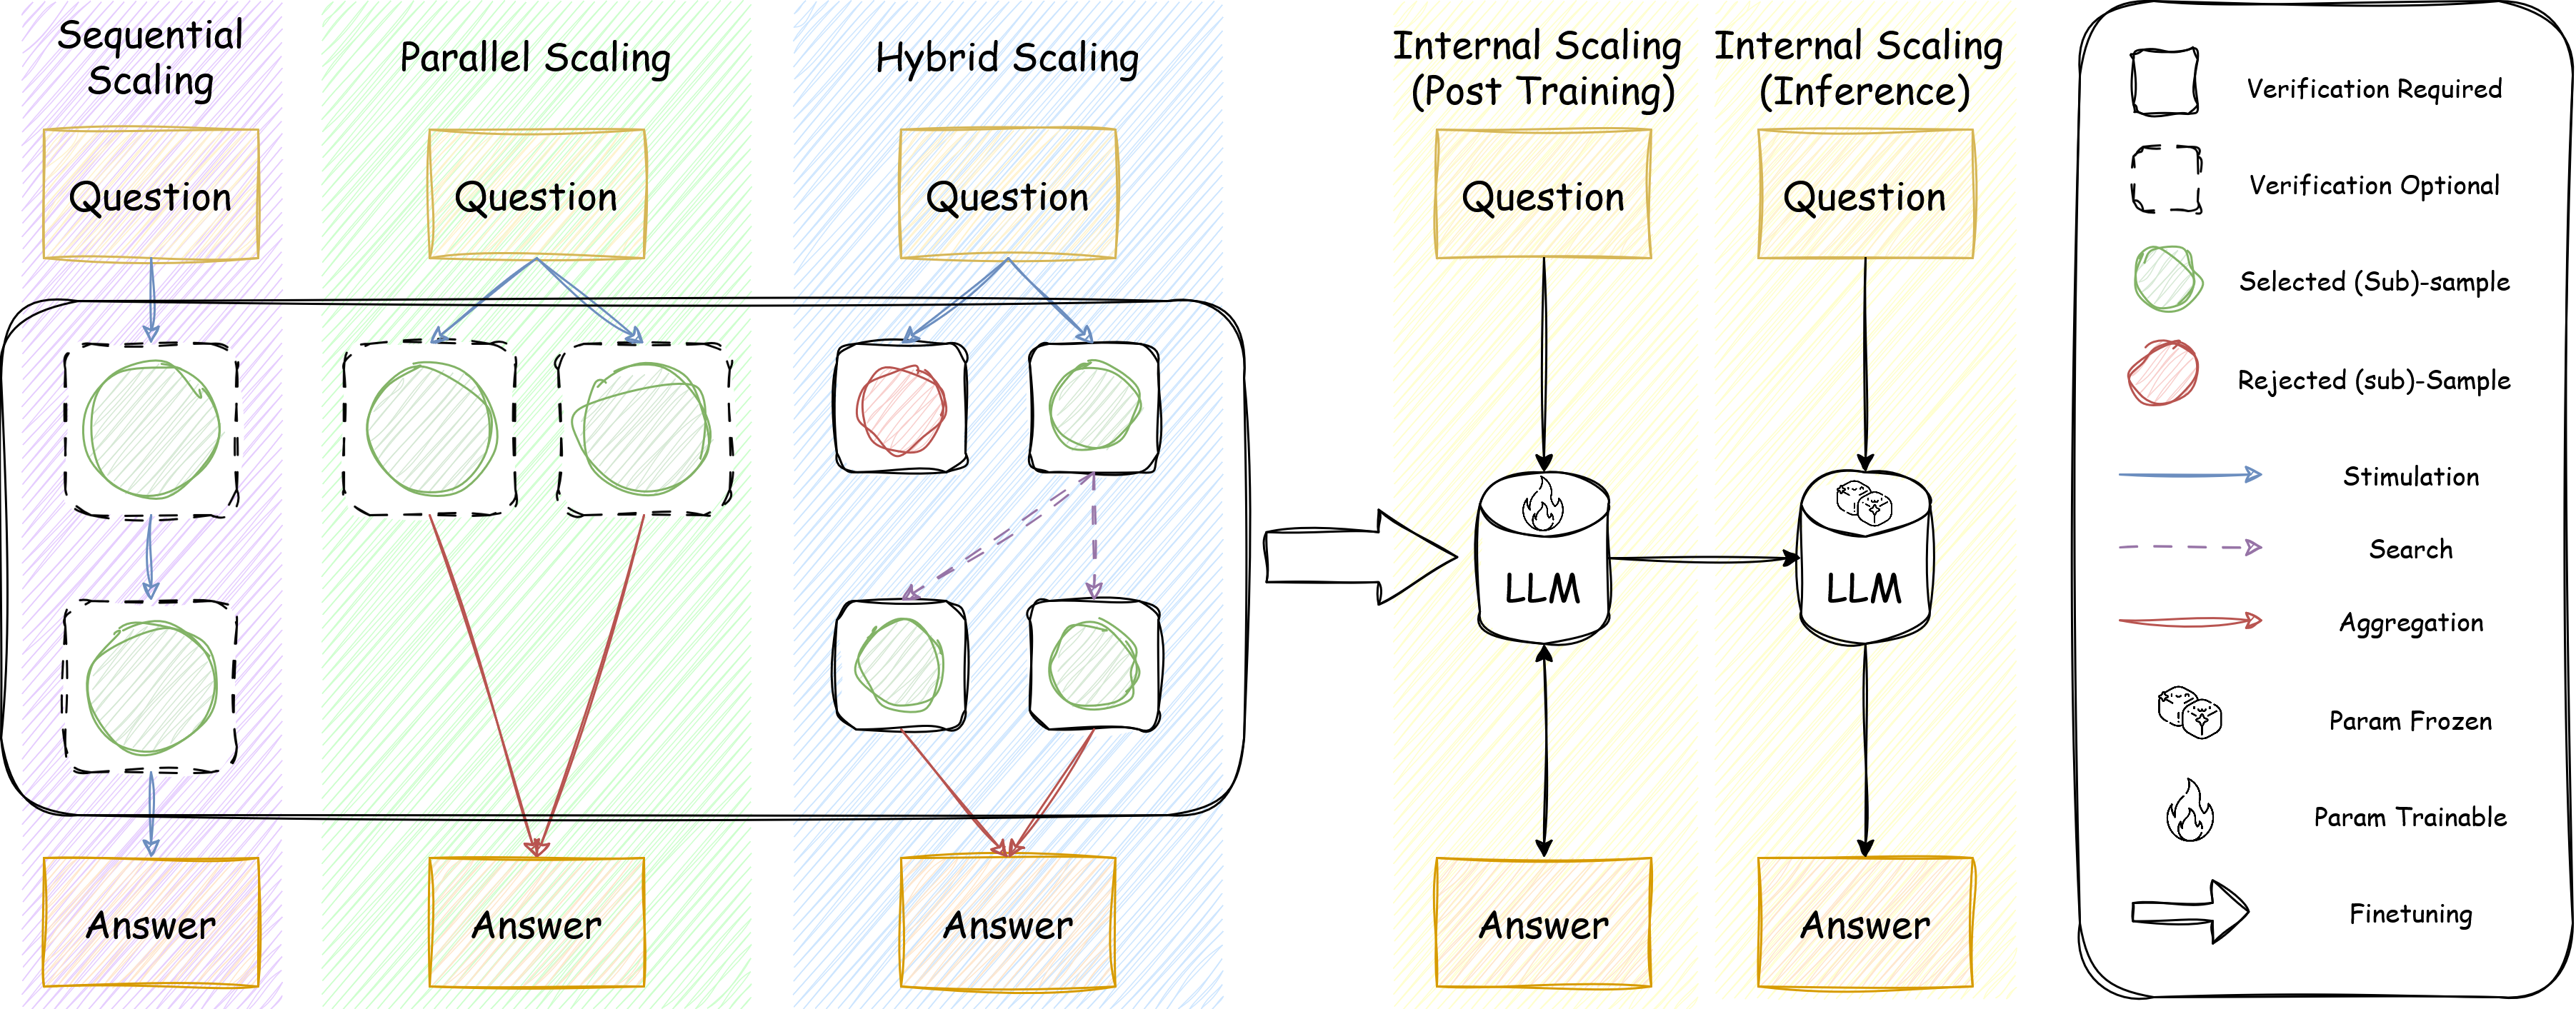
\includegraphics[width=0.98\linewidth]{figures/TTS-how.png}
    \caption{A Visual Map and Comparison: From \textit{What to Scale} to \textit{How to Scale}.}
    \label{fig:illustration}
\end{figure}

Unlike training-based approaches, which adjust the model’s parameters offline, inference-based approaches dynamically adjust computation during deployment. This paradigm includes four essential components: (i) \textit{Stimulation}, which encourages the model to generate longer or multiple candidate outputs; (ii) \textit{Verification}, which filters or scores outputs based on correctness or other criteria; (iii) \textit{Search}, which systematically explores the sample space; and (iv) \textit{Aggregation}, which consolidates multiple outputs into the final output. These four components are often used in combination to allocate test-time computation more effectively and boost performance on complex reasoning tasks. In the following sections, we provide detailed discussions of each component.


\subsubsection{Stimulation}
\label{subsec:stimulation}

Stimulation techniques are the first step in encouraging the model to allocate more computation to thinking. It basically stimulates the LLM to generate (i) longer samplers and (ii) more samples instead of generating single and short samples via naive prompting. This includes several key approaches:


\paragraph{Prompt Strategy.} Instead of allowing the model to generate an answer directly, one way to stimulate the scaling of LLM during test time is through the prompt. This behavior requires the backbone LLM's ability to follow instructions. For instance, prompts can guide the model toward step-by-step reasoning. Simple modifications such as adding explicit instructions (\eg, ``Please think step by step.'') can improve the model’s ability to break down complex problems into intermediate steps~\citep{lightman2023let}. This strategy ensures more deliberate and structured thought generation by shaping the reasoning process at the input level. Other techniques such as ~\cite{wei2022chain, ranaldi2025improvingchainofthoughtreasoningquasisymbolic} also rely on explicitly stating the requirements in the prompt to stimulate samples during the \TTS.

\paragraph{Decode Strategy} Rather than passively accepting the model’s default output behavior, this approach modifies the decoding process to encourage LLM to generate longer, more detailed samples adaptively. Techniques such as 
% length penalties, token constraints, or iterative response expansion 
injecting filler token~\citep{pfau2024lets}, adaptively injecting predefined injection phrase~\citep{jin2020diseasedoespatienthave}, forcing scaling budget~\citep{muennighoff2025s1}, enforcing intermediate generation~\citep{li2025draftsanswersunlockingllm}, or predictive decoding~\citep{ma2025nonmyopic} allow the model to modify its distribution progressively. Enforcing extended reasoning at the output level enables the model to think longer and generate more comprehensive solutions without requiring additional external guidance.

\paragraph{Latent Strategy}  Unlike strategies that rely on token-level instructions or output expansion, latent strategies encourage deeper or recurrent thinking within the hidden representations themselves, effectively scaling up test-time computation through continuous internal states. For example, \citet{hao2024training} propose a paradigm where the model completes reasoning steps entirely in hidden space before producing the final answer; \citet{kong2025scalablelanguagemodelsposterior} introduce a latent-thought framework that conditions text generation on an inferred latent variable to guide more thorough or expansive reasoning, while \citet{shen2025codicompressingchainofthoughtcontinuous} show that compressing CoT into continuous embeddings can preserve intermediate reasoning fidelity without lengthy textual traces. Other approaches~\citep{saunshi2025reasoninglatentthoughtspower} harness \emph{looped} or \emph{recurrent} inference to repeatedly refine hidden states, effectively unfolding multiple ``thinking iterations'' in a single forward pass. 


\paragraph{Self-Repetition Strategy} Apart from generating longer samples, another way to stimulate the LLM is to generate multiple samples instead of individual ones. One commonly adopted strategy is to prompt the LLM repeatedly during the decoding stage, commonly known as self-repetition~\citep{wang2023selfconsistency}. Another strategy is to prompt the LLM sequentially, in order to mimic refinement process~\citep{madaan2023selfrefine} or correlation under constraint~\citep{ferraz2024llmselfcorrectiondecrimdecompose}. 

\paragraph{Mixture-of-Model Strategy} Gathering the ``wisdom of the crowd'' can move beyond repeated sampling from a single model to coordinated sampling across multiple models. These LLMs can play either homogeneous roles~\citep{wang2025mixtureofagents} or heterogeneous roles~\citep{chen2024braininspiredtwostageapproachenhancing,he2025enhancingllmreasoningmultipath} during the process. By harnessing diverse perspectives, such multi-model strategy not only increases the coverage of possible solutions but also improves the system’s overall robustness. 

\begin{table*}[!htbp]
    \centering
    \resizebox{0.98\textwidth}{!}{
    \begin{tabular}{lll}
    \toprule
        \rowcolor{gray!10}
        \textbf{Category} & \textbf{Approach} & \textbf{Approach Description} \\
    \midrule
        & CoT~\citep{wei2022chain} & Contains a series of intermediate reasoning steps in prompts \\
        & Step-by-step~\citep{lightman2023let} & Stimulate step-by-step thinking via prompt \\
        & QuaSAR~\citep{ranaldi2025improvingchainofthoughtreasoningquasisymbolic} & Decompose CoT into Quasi-Symbolic Language \\
        & CoD~\citep{xu2025chaindraftthinkingfaster} & Generate concrete representations and distill into concise equation \\
        & Hint-infer~\citep{li2025startselftaughtreasonertools} & Inserting artificially designed hints in the prompt \\
        & Think~\citep{li2025startselftaughtreasonertools} & Prompt LLM with ``Think before response`` \\
        \multirow{-6}{*}{\textbf{Prompt}}
        & Think About World~\citep{jin2024impact} & Prompt LLM with ``Think About the World`` to enforce larger inference \\
        % & Coconut~\citep{hao2024training} & CoT without explicit decoding into tokens during the process \\
    \midrule
        \rowcolor{gray!10}
        & Filler-token~\citep{pfau2024lets} & uses arbitrary, irrelevant filler tokens before answering \\
        \rowcolor{gray!10}
        & Budget-forcing~\citep{muennighoff2025s1} & suppress the generation of the end-of-thinking token \\
        \rowcolor{gray!10}
        %& LTV~\citep{kong2025scalablelanguagemodelsposterior} & decode according to latent thought following prior model \\
        %\rowcolor{gray!10}
        & AFT~\citep{li2025draftsanswersunlockingllm} & iteratively aggregating proposals and aggregate for future proposals \\
        \rowcolor{gray!10}
        & Predictive-Decoding~\citep{ma2025nonmyopic} & re-weight decoding distribution given evaluation of foresight\\
        \rowcolor{gray!10}\multirow{-6}{*}{\textbf{Decode}} 
        & Adaptive Injection~\citep{jin2025wellthinkingenhancingllm} & Injecting a predefined injection phrase under certain condition \\
    \midrule
        & Coconut~\citep{hao2024training} & Perform chain-of-thought in hidden space without explicit token generation \\
        & CoDI~\citep{shen2025codicompressingchainofthoughtcontinuous} & Compress chain-of-thought into continuous vectors via self-distillation \\
        & Looped (Recurrent) Transformers~\citep{saunshi2025reasoninglatentthoughtspower} & Unroll model depth at inference by repeatedly refining hidden states \\
        & Heima~\citep{shen2025efficientreasoninghiddenthinking} & Encode each reasoning step into a single latent token to reduce output length \\
        \multirow{-5}{*}{\textbf{Latent}}
        & LTV~\citep{kong2025scalablelanguagemodelsposterior} & Introduce a latent thought variable to guide text generation \\
    \midrule
        \rowcolor{gray!10}
        & Self-Repetition~\citep{wang2023selfconsistency} & prompt LM in parallel \\
        \rowcolor{gray!10}
        & Self-Refine~\citep{madaan2023selfrefine} & Naively prompt LM to iteratively refine answer \\
        \rowcolor{gray!10}\multirow{-3}{*}{\textbf{Self-Repetition}}
        & DeCRIM~\citep{ferraz2024llmselfcorrectiondecrimdecompose} & Self-correlation for multi-constrained instruction following \\
    \midrule
        & MoA~\citep{wang2025mixtureofagents} & Prompt different models in parallel and iteratively improve \\
        & RR-MP~\citep{he2025enhancingllmreasoningmultipath} & Propose Reactive and Reflection agents to collaborate \\
        & BRAIN~\citep{chen2024braininspiredtwostageapproachenhancing} & Propose frontal \& parietal lobe model to inspire brain \\
        \multirow{-4}{*}{\textbf{Mixture-of-Model}}
        & Collab~\citep{chakraborty2025collab} & Propose decoding strategies to leverage multiple off-the-shelf aligned LLM policies \\
    \bottomrule
    \end{tabular}}
    \caption{Summary of Certain Stimulation Techniques.}
    \label{tab:stimulation}
\end{table*}


\subsubsection{Verification}
\label{subsec:verification}
Verifying the correctness and consistency of LLM during the test-time scaling is also crucial. The verification process plays an important role in the test-time scaling, as a solid verification process can be adapted to: 
\begin{itemize}
    \item directly selects the output sample among various ones, under the \textit{Parallel Scaling} paradigm;
    \item guides the stimulation process and determines when to stop, under the \textit{Sequential Scaling} paradigm;
    \item serves as the criteria in the search process, which we will discuss in Section~\ref{subsec:search};
    \item determines what sample to aggregate and how to aggregate them, e.g., weights, which we will discuss in Section~\ref{subsec:aggregation}.
\end{itemize}
Usually, there are two types of verifications, as shown below:

\paragraph{Outcome Verification.}
%Output verification approaches directly verify the sample outcome. \citet{cobbe2021training} initially proposes to train additional verifiers instead of fine-tuning models on mathematical tasks. 
Outcome verification plays a crucial role in ensuring the correctness and consistency of generated outputs. Common approaches include using a separate verifier model to score multiple candidate answers (\eg,\citet{cobbe2021training}), employing self-consistency, voting mechanisms~\citep{wang2023selfconsistency} and discriminator LM~\citep{chen2024tree} and leveraging tool-assisted~\citep{gou2024critic} or heuristic checks~\citep{deepseek-r1} in domains such as math and code generation. 
For specific task problems, such as trip planning, functional scoring~\citep{lee2025evolvingdeeperllmthinking} is also adopted for verifying the proposed plans. 
Instead of formulating the outcome verification as a classification problem, \citet{zhang2025generativeverifiersrewardmodeling} exploits the generative ability of LLM and proposes to reformulate the outcome verification process as a next-token prediction task.
\citet{li2025learningreasonfeedbacktesttime} formulate the feedback utilization as an optimization problem and adaptive propagate information between samples.

Apart from single criteria, certain outcome verification approaches verify the quality of the simulated samples from multiple perspectives. 
\citet{liu2023plan} conducts both (i) passive verification from external tools and (ii) active verification via a rethinking mechanism to justify each sample.
\citet{zhang2024wrongofthoughtintegratedreasoningframework} follows a similar idea and proposes to verify each sample from three aspects: Assertion, Process, and Result.
\citet{lifshitz2025multiagent} further extends the number of verification agents to an arbitrary number and decouples the semantic criteria with verification agents. 
\citet{parmar2025plangenmultiagentframeworkgenerating} and \citet{saadfalcon2024archonarchitecturesearchframework} also propose a verification agent to score each sample considering various factors, respectively. \citet{saadfalcon2024archonarchitecturesearchframework} additionally proposes a unit test-based verification approach.
We provide a detailed technical categorization in the Appendix~\ref{app:outcome_verification}.
%Table~\ref{tab:outcome_verification_methods} summarizes the main outcome-based verification methods, categorizing them by approach and providing brief descriptions.

% Output verification can also be extended to guide the decoding process during stimulation~\citep{yu2024ovm}.

\paragraph{Process Verification.}
Process verification approaches verify the sample outcomes and the process of obtaining such an outcome. They are commonly adopted in tasks with formal, deductive processes, such as reasoning, coding, or mathematics. They are also known as the process reward model (PRM) or state verification. \citet{lightman2023let} processes to train a PRM as a step-level verification on mathematical tasks. \citet{yao2023tree} processes an LM-based state verifier as guidelines for searching the samples under the tree structure. \citet{zhang2024chain} further tunes these preference data into LLM and enables CoT structure during test time. Instead of training an external verifier, \citet{xie2023selfevaluation} prompts the same LM to evaluate the current step given all previous ones. \citet{hosseini2024vstartrainingverifiersselftaught} proposes to train the verifier with both accurate and inaccurate generated data.
Although LM-based process verifiers can be easily integrated, they may yield unreliable verification, especially for complex problems with long processes. \citet{ling2023deductive} decomposes the verification process in a deductive manner. Hence, the verifier only needs to verify a few statements within the long thought chain. \citet{yu2024siamselfimprovingcodeassistedmathematical} is based on similar intuition but instead focuses on code-aided mathematical reasoning tasks with the critic model iteratively. \citet{li2025startselftaughtreasonertools} instead relies on the external toolbox, such as code interpreters, to verify the process. 


\begin{table*}[!htbp]
    \centering
    % \rowcolors{1}{}{gray!10}
    \resizebox{0.98\textwidth}{!}{
    \begin{tabular}{lll}
    \toprule
        \rowcolor{gray!10}
        \textbf{Category} & \textbf{Approach} & \textbf{Approach} Description \\
    \midrule
        \multirow{11}{*}{\textbf{Outcome}}
        & Naive ORM~\citep{cobbe2021training} & Naively process to train solution-level and token-level verifiers on labeled-dataset \\
        & OVM~\citep{yu2024ovm} & Train a value model under outcome supervision for guided decoding \\
        & Heuristic~\citep{deepseek-r1} & Heuristic check for domain-specific problems \\
        & Functional~\citep{lee2025evolvingdeeperllmthinking} & Functional scoring for task-specific problems \\
        & Bandit~\citep{sui2025metareasonerdynamicguidanceoptimized} & Train a bandit algorithm to learn how to verify \\
        & Generative Verifier~\citep{zhang2025generativeverifiersrewardmodeling} & Exploit the generative ability of LLM-based verifiers via reformulating the verification \\
        & Self-Reflection Feedback~\citep{li2025learningreasonfeedbacktesttime} & formulate the feedback utilization as an optimization problem and solve during test-time \\
        & Discriminator~\citep{chen2024tree} & SFT a domain-specific LM as a discriminator \\
        & Unit Test~\citep{saadfalcon2024archonarchitecturesearchframework} & Verify each sample as unit tests \\
        & XoT~\citep{liu2023plan} & Passive verification from external tools and Activate verification via re-thinking \\
        & WoT~\citep{zhang2024wrongofthoughtintegratedreasoningframework} & Multi-Perspective Verification on three aspects: Assertion, Process, and Result \\
        & Multi-Agent Verifiers~\citep{lifshitz2025multiagent} & Multi-Perspective Verification without explicit semantic meanings \\
    \midrule
        \rowcolor{gray!10}
        & Naive PRM~\citep{lightman2023let} & SFT an LM as a PRM on each reasoning step over mathematical tasks \\
        \rowcolor{gray!10}
        & State Verifier~\citep{yao2023tree} & SFT an LM as a state verifier and evaluate states either independently or jointly \\
        \rowcolor{gray!10}
        & Deductive PRM~\citep{ling2023deductive} & Deductively verify a few statements in the process \\ 
        \rowcolor{gray!10}
        & Self-Evaluation~\citep{xie2023selfevaluation} & Prompting the same LM to evaluate the current step given previous ones \\
        \rowcolor{gray!10}
        & PoT~\citep{chen2023program} & delegate computation steps to an external language interpreter \\
        \rowcolor{gray!10}
        & Tool~\citep{li2025startselftaughtreasonertools} & Relies on external toolbox for verification \\
        \rowcolor{gray!10}\multirow{-7}{*}{\textbf{Process}}
        & V-STaR~\citep{hosseini2024vstartrainingverifiersselftaught} & Verifier trained on both accurate and inaccurate self-generated data \\
    \bottomrule
    \end{tabular}}
    \caption{Summary of Certain Verification Techniques.}
    \label{tab:verification}
\end{table*}




\subsubsection{Search}
\label{subsec:search}

Search is also a frequently used component during the test-time scaling. LLMs pre-trained on vast amounts of online data, can be viewed as a compression of real-world knowledge. However, standard inference tends to underutilize their capacity. Search, being a classic yet working technique in retrieving relevant information from vast databases, can be utilized to fully exploit the capability of LLMs by exploring their potential options in a structured manner. Existing test-time scaling approaches based on search techniques demonstrate significant performance increases over complex tasks, such as complex mathematics, etc.

\citet{yao2023tree} explores the potential of search by decomposing the output samples into multiple thoughts and organizing them in a tree structure. Based on only Naive tree search algorithms, such as depth-first search and breath-first search, it demonstrates superior performance on reasoning tasks. 
Monte-Carlo Tree Search~\citep{coulom2006efficient}, being a classical and powerful search algorithm, also shines its light on better exploiting the hidden knowledge of LLMs.
\citet{chaffin2022ppl} adopts MCTS during the decoding stage guided by discriminators for constrained textual generation.
\citet{zhang2023planning} further extends the MCTS to enhance the planning ability in code generation via looking ahead.
\citet{tian2024toward} incorporates the MCTS as a critical component in the self-improving framework for LLM.
\citet{wan2024alphazero} tailors the search algorithm to tackle problems requiring long-horizon planning and deep tree structure for searching.
\citet{chen2024tree} further identifies that discriminators are the key bottleneck in search-enhanced planning.
\citet{gandhi2024streams} systematizes the search process in a unified language and proposes to train an LLM with data and feedback from the search process.
\citet{wu2024scaling} empirically analyzes various search algorithms and designs a reward-balanced search algorithm toward Pareto-optimal test-time scaling.
\citet{beenching2024scaling} further extends the beam search by incorporating diversity consideration.

Apart from searching within the tree structure, \citet{Besta2024graph} models the output as a graph search problem.
\citet{xie2023selfevaluation} proposes a stochastic beam search solution based on self-evaluation for reasoning tasks.
\citet{pan2025coatchainofassociatedthoughtsframeworkenhancing} enhances MCTS with proposed associative memory to dynamically update its knowledge base.
\citet{li2025reasoningaslogicunitsscalingtesttimereasoning} proposes to solve the reasoning process as constructing a control flow graph with each node indicating a logic unit.

% To enhance the efficiency and accuracy of test-time scaling, search techniques guide the model toward optimal solutions by systematically exploring the sample space. This includes two key approaches:
% \paragraph{Trajectory Strategy} Instead of generating a single reasoning path, the model actively explores multiple trajectories, adjusting its steps dynamically based on intermediate signals. This approach includes methods like beam search and Monte Carlo Tree Search (MCTS), allowing the model to prioritize promising reasoning paths while pruning less relevant ones. By adaptively allocating computational resources to high-value trajectories, this strategy enhances both depth and efficiency in problem-solving.
% \paragraph{Verifying Strategy} Rather than relying solely on the model’s initial output, this approach incorporates an external verification process to assess and refine responses. This may involve a reward model, consistency checks, or execution-based validation, ensuring that only reliable and logically sound answers are retained. By integrating feedback loops and validation mechanisms, the verifying strategy reduces hallucinations and increases confidence in the final output.



\subsubsection{Aggregation}
\label{subsec:aggregation}
Aggregation techniques consolidate multiple solutions into a final decision to enhance the reliability and robustness of model predictions at test time. 
Based on how the final output is generated, we empirically categorize them into two key classes: (i) Selection, which selects the best-performed sample among all candidates, where the selection criteria may vary across different approaches; and (ii) Fusion, which fuse multiple samples into one though tricks like weighting or generation.

\paragraph{Selection} 
In this category, the aggregation process can be viewed as a selection problem. 
One well-known example is to select the most consistent answer, commonly known as \textit{self-consistency}. \citet{wang2023selfconsistency} improves accuracy by leveraging statistical redundancy—if different reasoning paths converge to the same conclusion, the answer is more likely to be correct. Self-consistency effectively reduces variance in model outputs and mitigates occasional hallucinations. However, as the final output is voted based on consistency, inaccurate and low-quality samples would inevitably influence the output quality. Therefore, various approaches are proposed to filter the candidates before voting. \citet{chen2024are} incorporates an LM as a filter, while \citet{wu2025lessunderstandingchainofthoughtlength} proposes a Length-filtered vote, where prediction uncertainty is adopted as a proxy to filter reliable CoT length. 

Best-of-N~\citep{irvine2023rewarding} follows the same process but replaces the self-consistency criteria with scalar scores generated by external verifiers. 
\citet{song2024good} further demonstrates that best-of-N on small LLMs can yield competitive performance against SOTA propriety models.
\citet{munkhbat2025selftrainingelicitsconcisereasoning} attaches a few-conditioning filtering before the best-of-N selection. This aims to alleviate its sample inefficiency and achieves significant length reduction.
Motivated by particle filtering, \citet{puri2025probabilisticinferenceapproachinferencetime} proposes to consider filtering upon the samples.
\citet{sessa2024bondaligningllmsbestofn} went one step further in reducing sample inefficiency. It tunes the best-of-N results into the LM via RLHF.
With the blooming of the agentic approach, \citet{parmar2025plangenmultiagentframeworkgenerating} proposes a selection agent considering complex factors with both historical and current status.
Apart from selecting samples from one single LM, \citet{ong2025routellm} views the selection of samples generated by weak and strong LLMs as a routing problem and proposes constraints on computation costs. 

\paragraph{Fusion}
Directly selecting the final output sample among candidates may yield unsatisfactory results, especially when the sample quality of candidates is low. Fusion approaches propose to merge multiple samples into one to solve such a problem.
\citet{brown2024large} and \citet{li2023making} extend the idea from Best-of-N and weigh each sample by its score from external verifiers.
\citet{jiang2023llm}, on the other hand, directly prompts another LLM as a summarizer to merge multiple selected samples.
\citet{li2025llmsgeneratebetteranswer} shares similar intuition by replacing the majority voting in self-consistency~\citep{wang-etal-2024-math} with generative self-aggregation.
\citet{li2025reasoningaslogicunitsscalingtesttimereasoning} also adopts LLM as the synthesizer, given the intermediate consideration in previous steps.


\begin{table}[!htbp]
    % \rowcolors{2}{gray!10}{white}
    \centering
    \resizebox{0.98\textwidth}{!}{
    \begin{tabular}{l|l|c|l|l}
    \hline
        \rowcolor{gray!10}
        Category & Approach & External Verifier & Approach Description & Also Utilized in \\
    \hline
        & Majority Voting~\citep{wang2023selfconsistency} & \xmark & Select the most common sample & \cite{chen2024are} \\
        & Best-of-N~\citep{irvine2023rewarding} & \cmark & Select the highest scored sample & \cite{song2024good} \\
        & Few-shot BoN~\citep{munkhbat2025selftrainingelicitsconcisereasoning} & \cmark & BoN with few-shot conditioning \\
        \multirow{-4}{*}{Selection}
        & Agentic~\citep{parmar2025plangenmultiagentframeworkgenerating} & \xmark & agent considering both current and previous status \\
    \hline
        \rowcolor{gray!10}
        & Weighted BoN~\citep{li2023making} & \cmark & Weight each sample by its score & \cite{brown2024large} \\
        \rowcolor{gray!10} 
        & Synthesize~\citep{jiang2023llm} & \xmark & Fuse the selected samples via GenAI & \cite{wang2025mixtureofagents,li2025reasoningaslogicunitsscalingtesttimereasoning} \\
        \rowcolor{gray!10} \multirow{-3}{*}{Fusion}
        & Ensemble Fusion~\citep{saadfalcon2024archonarchitecturesearchframework}& \xmark & Conduct ensemble before fusion & \\
    \hline
    \end{tabular}}
    \caption{Summary of Certain Aggregation Techniques. BoN stands for Best-of-N.}
    \label{tab:aggregation}
\end{table}


% Based on the sample to aggregate, these approaches can be categorized into two key classes and summarized in Table~\ref{tab:aggregation}.
% \paragraph{Self-Repetition} Instead of relying on a single reasoning trajectory, the model samples multiple independent CoTs from the sample basic LLM. One example is to select the most consistent answer, commonly known as \textit{self-consistency}~\citep{wang2023selfconsistency}. This approach improves accuracy by leveraging statistical redundancy—if different reasoning paths converge to the same conclusion, the answer is more likely to be correct. Self-consistency effectively reduces variance in model outputs and mitigates occasional hallucinations. Other methods, including Best-of-N~\citep{irvine2023rewarding} and its variants~\citep{brown2024large}, rely on external verifiers to score each sample and output the best-performed sample.

% \paragraph{Mixture of Models} Instead of relying on a single model, multiple models perform repeated sampling during the test-time scaling. This could further expand coverage and ensure a more comprehensive exploration of possible solutions, as different models tend to show different strengths on various tasks~\citep{jiang2023llm, zhang2024collaborative}. This paradigm enables diverse perspectives to contribute to the final answer, fostering a more reliable decision-making process.

